\documentclass{beamer}

\usepackage{ucs}
\usepackage[utf8]{inputenc}
\usepackage[T1]{fontenc}

\usepackage[ngerman]{babel}

\usetheme{Madrid}

\title{Git Präsentation - Part 1}
\author{Tobias Meier}
\institute{GDW Orga}
\date{\today}

\begin{document}

\begin{frame}
\titlepage
\end{frame}

\begin{frame}
\frametitle{Outline}
\tableofcontents[pausesections]
\end{frame}

\section{Versionsverwaltung}
\begin{frame}
	\frametitle{Versionsverwaltung}
	\begin{definition} <1->
		Eine Versionsverwaltung ist ein System, das zur Erfassung von Änderungen an Dokumenten oder Dateien verwendet wird. Alle Versionen werden in einem Archiv mit Zeitstempel und Benutzerkennung gesichert und können später wiederhergestellt werden.
	\end{definition}
	\begin{block} <2-> {Hauptaufgaben}
		\begin{itemize}
			\item <2-> Protokolierung der Änderungen
			\item <3-> Wiederherstellung von älteren Dateien
			\item <4-> Archivierung der einzelnen Stände eines Projektes
			\item <5-> Koordinierung des gemeinsamen Zugriffs von mehreren Entwicklern auf die Dateien
			\item <6-> Gleichzeitige Entwicklung mehrerer Branches eines Projektes
		\end{itemize}
	\end{block}	
\end{frame}


\section{Git}
\begin{frame}
	\frametitle{Git}
	\begin{block} <1-> {Eigenschaften}
		\begin{itemize}
			\item <1-> Dezentralität
			\begin{itemize}
				\item <1-> klon des kompletten Repositories lokal
			\end{itemize}
			\item <2-> Vieles läuft lokal
			\item <3-> Hashes statt Nummern
			\begin{itemize}
				\item <3-> dezentrale Architektur erlaubt keine fortlaufende Revisiond-Nummerierung
			\end{itemize}
			\item <4-> Lizenz: GNU GPLv2 (Frei Software / Open-Source-Software)
		\end{itemize}
	\end{block}
\end{frame}
\begin{frame}
	\frametitle{Git}
	\framesubtitle{4 Ebenen}
	\begin{columns}
		\column{0.5\textwidth}
			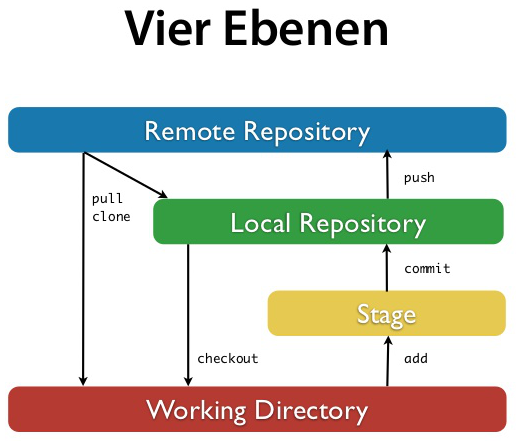
\includegraphics[scale=0.45]{./pictures/4_ebenen_git}
		\column{0.5\textwidth}
			\begin{block} <2-> {Remote Repository}
				Versionen des Projektes, welche sich im Internet oder Netzwerk befindet.
			\end{block}
			\begin{block} <3-> {Local Repository}
				Versionen des Projektes, welche sich lokal auf dem System befinden. 
			\end{block}
			\begin{block} <5-> {Stage}
				Eine Zwischenablage, aus der herraus man committen kann.
			\end{block}
			\begin{block} <4-> {Working Directory}
				Die eigentlichen Dateien
			\end{block}
	\end{columns}
\end{frame}

\section{git clone}
\begin{frame}
	\frametitle{clone}
	\begin{columns}
		\column{0.5\textwidth}
			\begin{itemize}
				\item <2-> alle Dateien werden in das working Directory kopiert
				\item <3-> alle remote Branches werden erstellt
				\item <4-> der default branche wird lokal erstellt (master)
			\end{itemize}	
		\column{0.5\textwidth}
			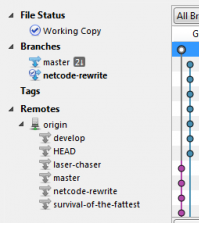
\includegraphics[scale=1.0]{./pictures/clone_branches}
	\end{columns}
\end{frame}
\begin{frame}
	\frametitle{clone}
	\begin{block} <1-> {Was benötigen wir zum clonen?}
		\begin{itemize}
			\item <1-> die URL, wo des remote repository liegt
			\begin{itemize}
				\item <1-> https://github.com/Lusito/GameDevWeek.git
			\end{itemize}
			\item <2-> einen lokalen Speicherplatz
		\end{itemize}
	\end{block}
\end{frame}
\begin{frame}
	\frametitle{clone}
	\centering {
		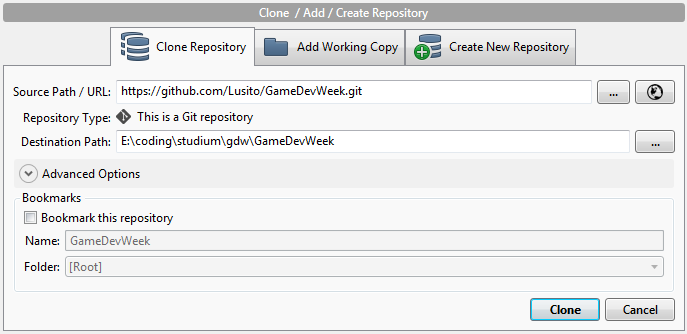
\includegraphics[scale=0.65]{./pictures/clone_sourceTree}
	}
\end{frame}

\section{Instalieren + Anwenden}
\begin{frame}
	Fröhliches Installieren, IDE aufsetzen und clonen!
\end{frame}
\end{document}